\documentclass[a4paper, 12pt]{article}
\usepackage[utf8]{inputenc}
\usepackage[margin=1 in]{geometry}
\usepackage{graphicx}
\graphicspath{{img/}}

\title{C\'omo escrbir a Documento de investigaci\'on efectivo}
\author{Jose Enrique Camacho Silvestre\thanks{ESSAYREVIEW}}
\date{\today}

\begin{document}
	\maketitle
	
	\section{Introducci\'on}
	This will be write after the sections: Methods, Results, Discussion and Conclusion.
	
	\section{Principios rectores de calidad de un documento de investigaci\'on}
		Existen varias formas de medir la calidad de un trabajo, sin embargo algunas siempre deber\'ian tomarse en cuenta, imaginemos esto como una lista de requerimientos minimos que debemos satisfacer para certificar un minimo de calidad a nuestro trabajo, el resto dependera de nuestra rigurisidad, estilo, y dominio del campo de investigaci\'on. Existen 4 factores de calidad coherencia, organizaci\'on, relevancia y claridad.
		
		\subsection{Coherencia}
			La coherencia trata con la continuidad, es decir el flujo. Algunos papers se leen sin problemas desde la primera oraci\'on hasta la \'ultima, debido a que toda la informaci\'on se formula de manera \emph{concisa} y todas las conexiones se expresan adecuadamente es decir que posee \emph{cohesi\'on}.
			 
			 Como se pudo observar la coherencia est\'a relacionada con la \emph{cohesi\'on} y la \emph{consistencia}:
			\subsubsection{Cohesi\'on}
				Es la fuerza que mantiene los elementos juntos, los enlaces textuales que mantienen unido a un texto y dejando fuera la informaci\'on innecesaria.
					\begin{figure}[h]
						\centering
						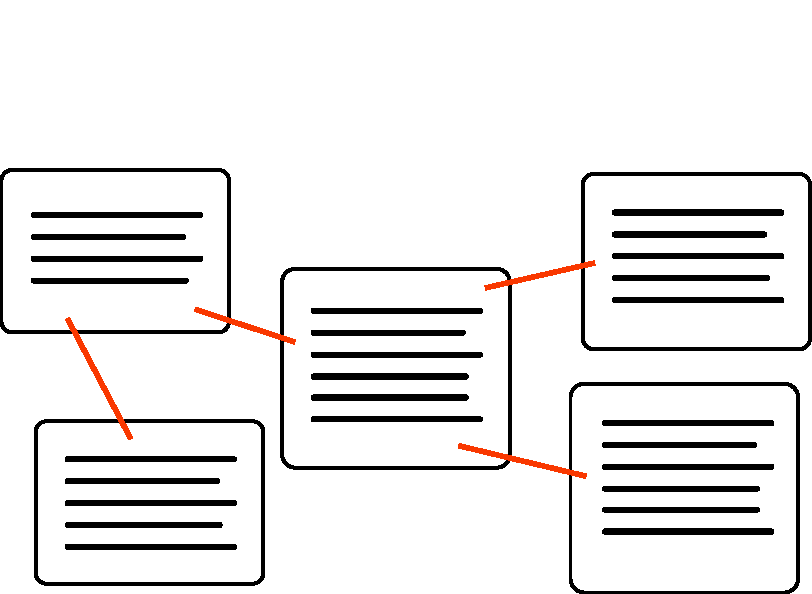
\includegraphics[width=0.4\textwidth]{cohesion.pdf}
						\caption{Figura 1: cohesi\'on}
						\label{fig: fig1}
					\end{figure}

			\subsubsection{Cosistencia}
				%Es la ausencia de contradicciones internas, es decir que se siguen los principios que se profesan, se debe seguir todo aquello que se manifiesta a lo largo del documento.
				Cuando se realizan manifiestos a lo largo del texto no deben existir contradicciones en el mismo (contradicciones internas), es decir se deben serguir los principios que se profesan. 
				
			Si nuestro documento cumple con ambas caracteristicas podemos hablar de un documento coherente.
		\subsection{Organizaci\'on}
			Se debe seguir una estructura en la investigaci\'on, una buena opci\'on es la estructara IMRD:
			\begin{center}
				\begin{enumerate}
					\item \textbf{I}ntroducci\'on
					\item \textbf{M}etodos
					\item \textbf{R}esultados
					\item \textbf{D}iscusi\'on
				\end{enumerate}
			\end{center}
			Ademas se exige que la informaci\'on este en su lugar correcto. A persar que nuestro documento sea coherente la informaci\'on debe estar organizida siguiendo nuestra estructura.
		\subsection{Relevancia}
			Existe bastante confusi\'on entre la relevancia y la Coherencia.
		\subsection{Claridad}
		
\end{document}


